\documentclass[border=10pt]{standalone}
\usepackage[T1]{fontenc}
\usepackage{times}
\usepackage{tikz}
\usetikzlibrary{shapes.geometric, arrows.meta, positioning, calc, fit, backgrounds}

\definecolor{inputblue}{RGB}{41,65,114}
\definecolor{processgreen}{RGB}{34,102,85}
\definecolor{scoreorange}{RGB}{153,84,34}
\definecolor{outputred}{RGB}{140,42,42}
\definecolor{lightgray}{RGB}{245,245,245}
\definecolor{midgray}{RGB}{210,210,210}
\definecolor{channelsem}{RGB}{225,238,248}
\definecolor{channelstr}{RGB}{232,245,233}

\begin{document}
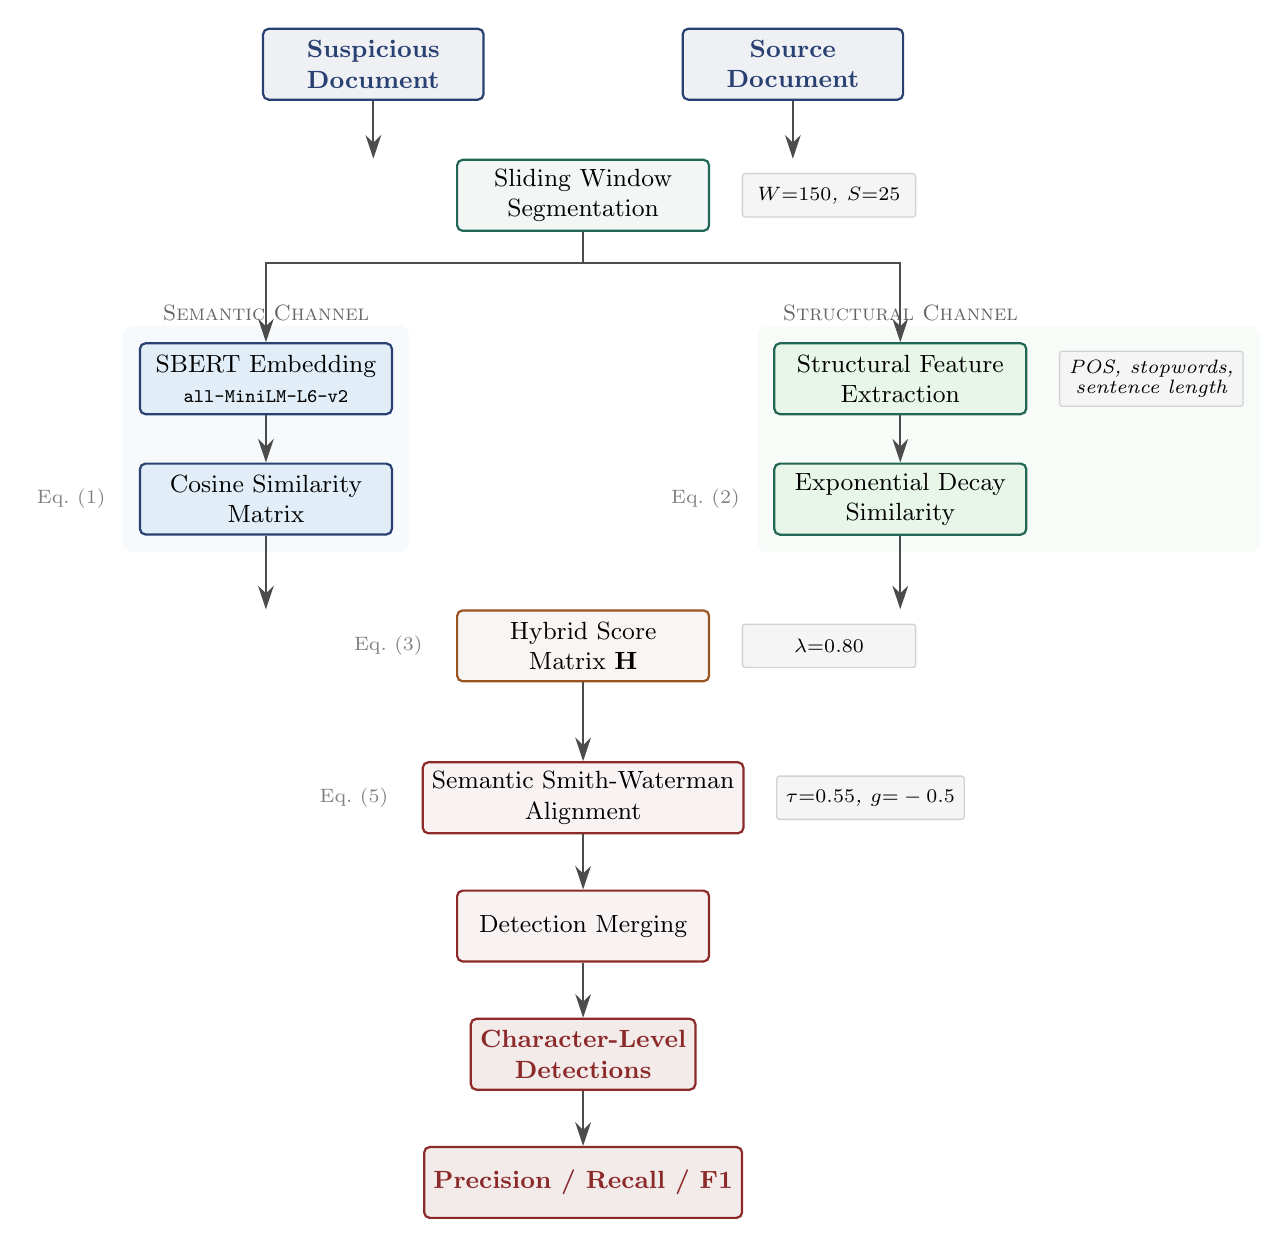
\begin{tikzpicture}[
    node distance=0.6cm and 1.2cm,
    >={Stealth[length=3mm, width=2mm]},
    % Block styles
    inputblock/.style={
        rectangle, draw=inputblue, fill=inputblue!8,
        text=inputblue, font=\small\bfseries,
        minimum width=2.8cm, minimum height=0.9cm,
        align=center, rounded corners=2pt,
        line width=0.8pt
    },
    processblock/.style={
        rectangle, draw=processgreen, fill=processgreen!6,
        text=black, font=\small,
        minimum width=3.2cm, minimum height=0.9cm,
        align=center, rounded corners=2pt,
        line width=0.8pt
    },
    scoreblock/.style={
        rectangle, draw=scoreorange, fill=scoreorange!6,
        text=black, font=\small,
        minimum width=3.2cm, minimum height=0.9cm,
        align=center, rounded corners=2pt,
        line width=0.8pt
    },
    alignblock/.style={
        rectangle, draw=outputred, fill=outputred!6,
        text=black, font=\small,
        minimum width=3.2cm, minimum height=0.9cm,
        align=center, rounded corners=2pt,
        line width=0.8pt
    },
    outputblock/.style={
        rectangle, draw=outputred, fill=outputred!10,
        text=outputred, font=\small\bfseries,
        minimum width=2.8cm, minimum height=0.9cm,
        align=center, rounded corners=2pt,
        line width=0.8pt
    },
    param/.style={
        rectangle, draw=midgray, fill=lightgray,
        text=black, font=\scriptsize\itshape,
        minimum width=2.2cm, minimum height=0.55cm,
        align=center, rounded corners=1pt,
        line width=0.5pt
    },
    grouplabel/.style={
        font=\footnotesize\scshape, text=black!60
    },
    arrow/.style={
        ->, line width=0.7pt, color=black!70
    },
    dashedarrow/.style={
        ->, line width=0.5pt, color=black!40, dashed
    },
]

% ===== STAGE 1: INPUT =====
\node[inputblock] (susp) {Suspicious\\Document};
\node[inputblock, right=2.5cm of susp] (src) {Source\\Document};

% ===== STAGE 2: WINDOWING =====
\node[processblock, below=1.2cm of $(susp)!0.5!(src)$] (window) {Sliding Window\\Segmentation};
\node[param, right=0.4cm of window] (winparam) {$W{=}150$, $S{=}25$};

% ===== STAGE 3: DUAL CHANNEL =====
% Semantic channel
\node[processblock, below left=1.4cm and 0.8cm of window, fill=channelsem, draw=inputblue] (sbert) {SBERT Embedding\\{\scriptsize\texttt{all-MiniLM-L6-v2}}};
\node[processblock, below=0.6cm of sbert, fill=channelsem, draw=inputblue] (cossim) {Cosine Similarity\\Matrix};

% Structural channel
\node[processblock, below right=1.4cm and 0.8cm of window, fill=channelstr, draw=processgreen] (feat) {Structural Feature\\Extraction};
\node[processblock, below=0.6cm of feat, fill=channelstr, draw=processgreen] (expdecay) {Exponential Decay\\Similarity};
\node[param, right=0.4cm of feat] (featparam) {\scriptsize POS, stopwords,\\[-1pt] \scriptsize sentence length};

% Channel labels
\node[grouplabel, above=0.15cm of sbert] {Semantic Channel};
\node[grouplabel, above=0.15cm of feat] {Structural Channel};

% ===== STAGE 4: FUSION =====
\node[scoreblock, below=1.4cm of $(cossim)!0.5!(expdecay)$] (hybrid) {Hybrid Score\\Matrix $\mathbf{H}$};
\node[param, right=0.4cm of hybrid] (hybparam) {$\lambda{=}0.80$};

% ===== STAGE 5: ALIGNMENT =====
\node[alignblock, below=1.0cm of hybrid] (sw) {Semantic Smith-Waterman\\Alignment};
\node[param, right=0.4cm of sw] (swparam) {$\tau{=}0.55$, $g{=}-0.5$};

% ===== STAGE 6: OUTPUT =====
\node[alignblock, below=0.7cm of sw] (merge) {Detection Merging};

\node[outputblock, below=0.7cm of merge] (output) {Character-Level\\Detections};

% ===== STAGE 7: EVALUATION =====
\node[outputblock, below=0.7cm of output] (eval) {Precision / Recall / F1};

% ===== ARROWS =====
% Input to windowing
\draw[arrow] (susp.south) -- ++(0,-0.3) -| (window.north -| susp);
\draw[arrow] (src.south) -- ++(0,-0.3) -| (window.north -| src);

% Windowing to channels
\draw[arrow] (window.south) -- ++(0,-0.4) -| (sbert.north);
\draw[arrow] (window.south) -- ++(0,-0.4) -| (feat.north);

% Within channels
\draw[arrow] (sbert) -- (cossim);
\draw[arrow] (feat) -- (expdecay);

% Channels to fusion
\draw[arrow] (cossim.south) -- ++(0,-0.35) -| (hybrid.north -| cossim);
\draw[arrow] (expdecay.south) -- ++(0,-0.35) -| (hybrid.north -| expdecay);

% Fusion to alignment
\draw[arrow] (hybrid) -- (sw);

% Alignment to merge to output
\draw[arrow] (sw) -- (merge);
\draw[arrow] (merge) -- (output);
\draw[arrow] (output) -- (eval);

% ===== EQUATION ANNOTATIONS =====
\node[font=\scriptsize, text=black!50, left=0.3cm of cossim] {Eq.~(1)};
\node[font=\scriptsize, text=black!50, left=0.3cm of expdecay] {Eq.~(2)};
\node[font=\scriptsize, text=black!50, left=0.3cm of hybrid] {Eq.~(3)};
\node[font=\scriptsize, text=black!50, left=0.3cm of sw] {Eq.~(5)};

% ===== BACKGROUND GROUPS =====
\begin{scope}[on background layer]
    % Semantic channel bg
    \node[fit=(sbert)(cossim), fill=channelsem!30, rounded corners=4pt, inner sep=6pt] {};
    % Structural channel bg
    \node[fit=(feat)(expdecay)(featparam), fill=channelstr!30, rounded corners=4pt, inner sep=6pt] {};
\end{scope}

\end{tikzpicture}
\end{document}
